%
% $RCSfile: logic_examples.tex,v $
%
% Copyright (c) 2002-2007. Christian Heller. All rights reserved.
%
% Permission is granted to copy, distribute and/or modify this document
% under the terms of the GNU Free Documentation License, Version 1.1 or
% any later version published by the Free Software Foundation; with no
% Invariant Sections, with no Front-Cover Texts and with no Back-Cover
% Texts. A copy of the license is included in the section entitled
% "GNU Free Documentation License".
%
% http://www.cybop.net
% - Cybernetics Oriented Programming -
%
% Version: $Revision: 1.1 $ $Date: 2007-08-01 13:59:00 $ $Author: christian $
% Authors: Christian Heller <christian.heller@tuxtax.de>
%

\section{Logic Examples}
\label{logic_examples_heading}
\index{CYBOL Logic Example Constructs}

The CYBOL implementation of logic models needs more detailed explanation, in
particular the use of special control structures as known from
\emph{Structured and Procedural Programming} (SPP).

%
% $RCSfile: operation_call.tex,v $
%
% Copyright (C) 2002-2008. Christian Heller.
%
% Permission is granted to copy, distribute and/or modify this document
% under the terms of the GNU Free Documentation License, Version 1.1 or
% any later version published by the Free Software Foundation; with no
% Invariant Sections, with no Front-Cover Texts and with no Back-Cover
% Texts. A copy of the license is included in the section entitled
% "GNU Free Documentation License".
%
% http://www.cybop.net
% - Cybernetics Oriented Programming -
%
% http://www.resmedicinae.org
% - Information in Medicine -
%
% Version: $Revision: 1.1 $ $Date: 2008-08-19 20:41:08 $ $Author: christian $
% Authors: Christian Heller <christian.heller@tuxtax.de>
%

\subsubsection{Operation Call}
\label{operation_call_heading}
\index{CYBOL Operation Call Example}

As stated previously, logic models may access and manipulate state models. The
simplest form of a logic model is an operation with associated input/ output
(i/o) state models. The following CYBOL knowledge template calls an \emph{add}
operation, handing over i/o parameters as \emph{properties} of the
corresponding \emph{part}:

\begin{scriptsize}
    \begin{verbatim}
<model>
    <part name="addition" channel="inline" abstraction="operation" model="add">
        <property name="summand_1" channel="inline" abstraction="integer" model="1"/>
        <property name="summand_2" channel="inline" abstraction="knowledge" model="domain.summand"/>
        <property name="sum" channel="inline" abstraction="knowledge" model="domain.result"/>
    </part>
</model>
    \end{verbatim}
\end{scriptsize}

The example nicely shows how state models can be given in various formats. The
\emph{summand\_1} is given as constant value, defined directly in the knowledge
template. Its type of abstraction is \emph{integer}. The \emph{summand\_2-} and
\emph{sum} parameters, on the other hand, are given as dot-separated references
to the runtime tree of knowledge models. Their type of abstraction is therefore
\emph{knowledge}.

%
% $RCSfile: algorithm_division.tex,v $
%
% Copyright (C) 2002-2008. Christian Heller.
%
% Permission is granted to copy, distribute and/or modify this document
% under the terms of the GNU Free Documentation License, Version 1.1 or
% any later version published by the Free Software Foundation; with no
% Invariant Sections, with no Front-Cover Texts and with no Back-Cover
% Texts. A copy of the license is included in the section entitled
% "GNU Free Documentation License".
%
% http://www.cybop.net
% - Cybernetics Oriented Programming -
%
% http://www.resmedicinae.org
% - Information in Medicine -
%
% Version: $Revision: 1.1 $ $Date: 2008-08-19 20:41:05 $ $Author: christian $
% Authors: Christian Heller <christian.heller@tuxtax.de>
%

\subsubsection{Algorithm Division}
\label{algorithm_division_heading}
\index{CYBOL Algorithm Division Example}

Compound logic models like \emph{Algorithms}, which SPP languages implement
using nested \emph{Blocks}, can be expressed in CYBOL as well. It does not
provide blocks in the classical sense, but its hierarchical structure allows to
subdivide compound knowledge templates, and to cascade compound logic as well
as primitive operations. The following example calls an addition operation,
before a compound algorithm, situated in an external CYBOL file, gets executed:

\begin{scriptsize}
    \begin{verbatim}
<model>
    <part name="addition" channel="inline" abstraction="operation" model="add">
        <property name="summand_1" channel="inline" abstraction="knowledge" model="domain.number_1"/>
        <property name="summand_2" channel="inline" abstraction="knowledge" model="domain.number_2"/>
        <property name="sum" channel="inline" abstraction="knowledge" model="domain.number_3"/>
    </part>
    <part name="algorithm" channel="file" abstraction="cybol" model="logic/algorithm.cybol"/>
</model>
    \end{verbatim}
\end{scriptsize}

%
% $RCSfile: simple_assignment.tex,v $
%
% Copyright (c) 2002-2007. Christian Heller. All rights reserved.
%
% Permission is granted to copy, distribute and/or modify this document
% under the terms of the GNU Free Documentation License, Version 1.1 or
% any later version published by the Free Software Foundation; with no
% Invariant Sections, with no Front-Cover Texts and with no Back-Cover
% Texts. A copy of the license is included in the section entitled
% "GNU Free Documentation License".
%
% http://www.cybop.net
% - Cybernetics Oriented Programming -
%
% Version: $Revision: 1.1 $ $Date: 2007-08-01 13:59:00 $ $Author: christian $
% Authors: Christian Heller <christian.heller@tuxtax.de>
%

\subsection{Simple Assignment}
\label{simple_assignment_heading}
\index{Simple Assignment Example}

CYBOL does not know \emph{Variables} as used in classical languages. All states
a system may take on are represented by just one \emph{Knowledge Tree}, which
applications may access in a defined manner (dot-separated knowledge paths).
Consequently, \emph{Assignments} are done differently in CYBOL than in
classical programming languages. All kinds of state changes go back to a
manipulation of the one knowledge tree:

\begin{scriptsize}
    \begin{verbatim}
<model>
    <part name="copy_value" channel="inline" abstraction="operation" model="copy">
        <property name="source" channel="inline" abstraction="knowledge" model="domain.name"/>
        <property name="destination" channel="inline" abstraction="knowledge" model="gui.name"/>
    </part>
    <part name="move_branch" channel="inline" abstraction="operation" model="move">
        <property name="source" channel="inline" abstraction="knowledge" model="address_1.phone"/>
        <property name="destination" channel="inline" abstraction="knowledge" model="address_2"/>
    </part>
</model>
    \end{verbatim}
\end{scriptsize}

The first operation in the example above copies a value between two branches of
the tree. Only primitive values can be copied. The second operation removes a
whole tree branch (referenced by the \emph{source} property) from one parent
node, and adds it to another (referenced by the \emph{destination} property).

%
% $RCSfile: loop_as_operation.tex,v $
%
% Copyright (c) 2002-2007. Christian Heller. All rights reserved.
%
% Permission is granted to copy, distribute and/or modify this document
% under the terms of the GNU Free Documentation License, Version 1.1 or
% any later version published by the Free Software Foundation; with no
% Invariant Sections, with no Front-Cover Texts and with no Back-Cover
% Texts. A copy of the license is included in the section entitled
% "GNU Free Documentation License".
%
% http://www.cybop.net
% - Cybernetics Oriented Programming -
%
% Version: $Revision: 1.1 $ $Date: 2007-08-01 13:59:00 $ $Author: christian $
% Authors: Christian Heller <christian.heller@tuxtax.de>
%

\subsection{Loop as Operation}
\label{loop_as_operation_heading}
\index{Loop as Operation Example}

\emph{Looping} is a major technique for the effective processing of whole
stacks of data. As many other control structures, it is simplified to a logic
operation, in CYBOL.

\begin{figure}[ht]
    \begin{center}
        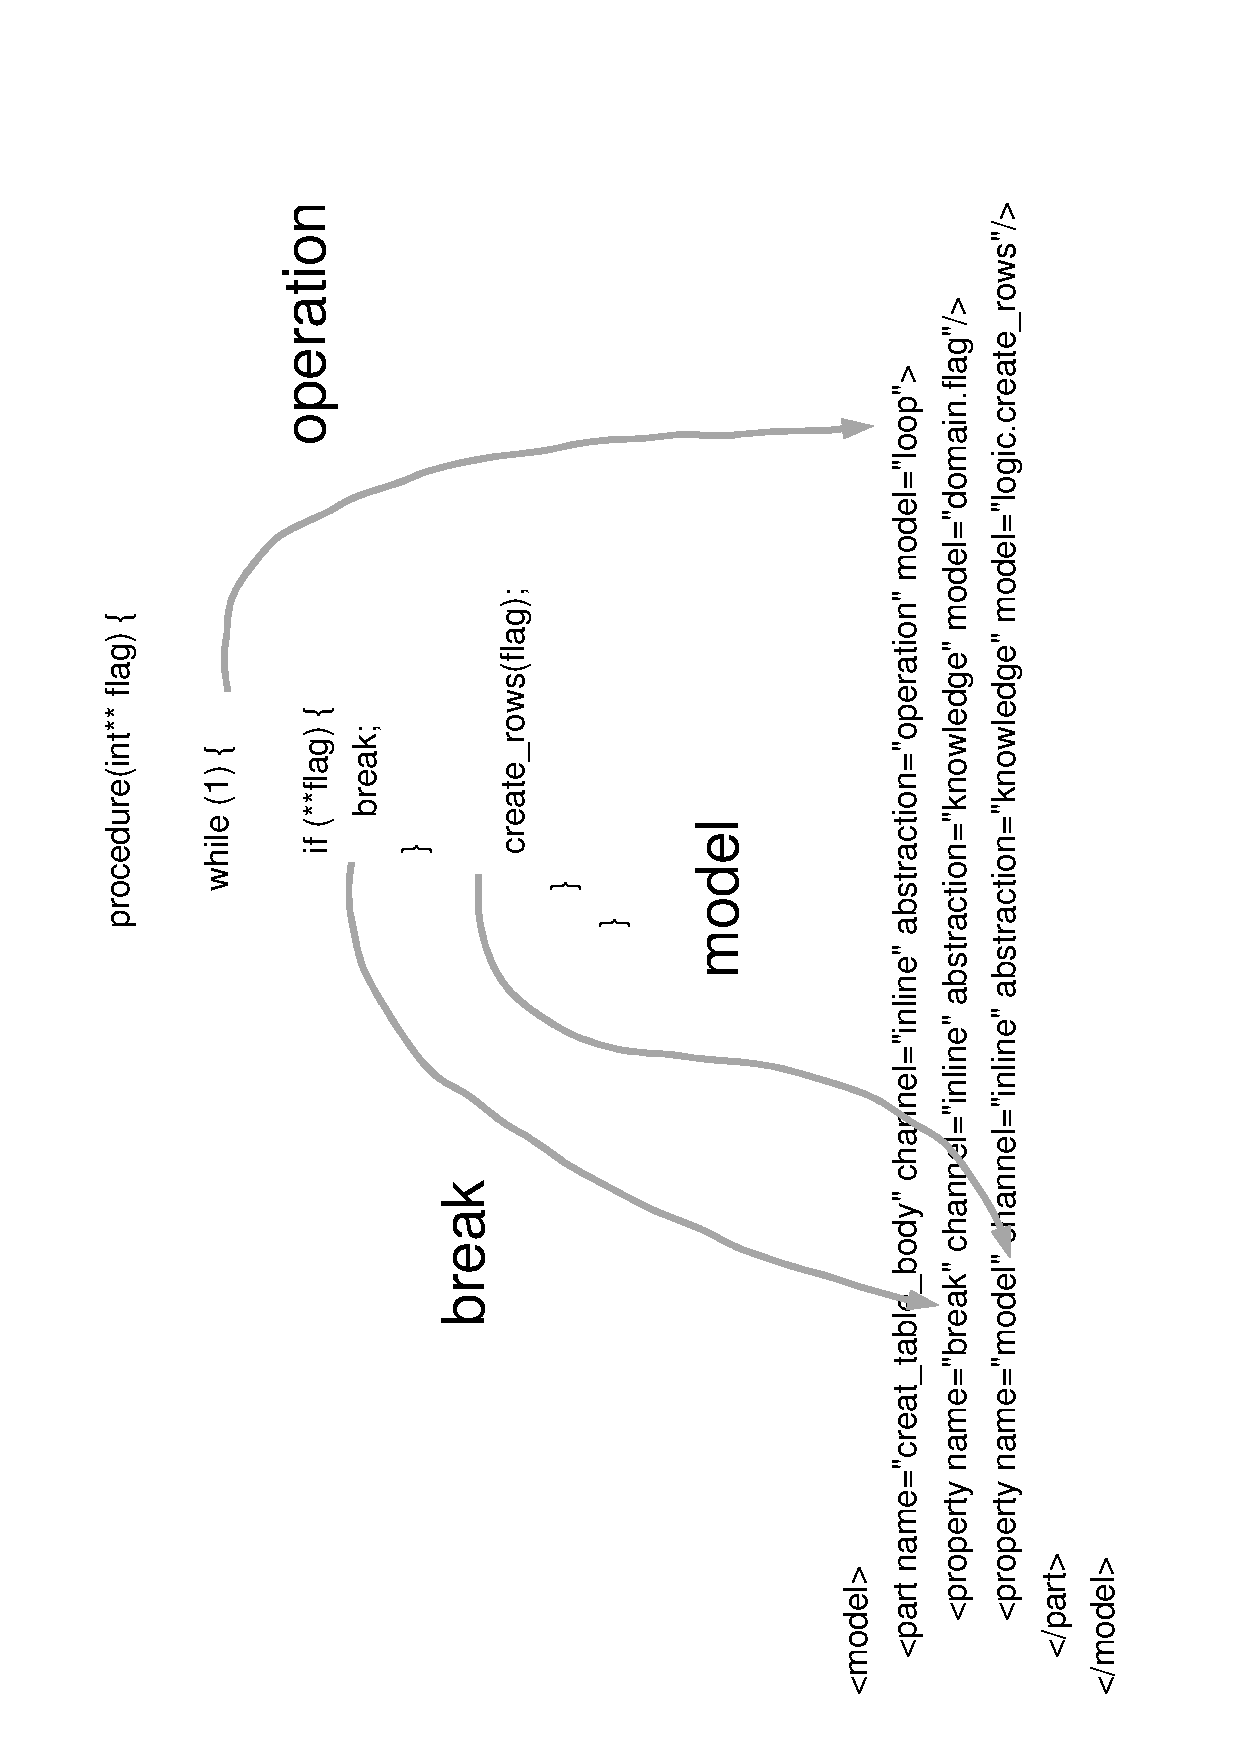
\includegraphics[scale=0.3,angle=-90]{graphics/cybolloop.pdf}
        \caption{Loop Control Structure and Elements in C and CYBOL}
        \label{cybolloop_figure}
    \end{center}
\end{figure}

The \emph{loop} operation needs two parameters to be functional: a \emph{break}
flag as means of interruption and a logic \emph{model} to be executed in each
loop cycle (figure \ref{cybolloop_figure}). An \emph{index} counting loop
cycles is not given, as it is in the responsibility of the logic \emph{model}
to manage that index, just like the setting of the \emph{break} flag,
internally. The following example dynamically creates a table consisting of a
number of rows:

\begin{scriptsize}
    \begin{verbatim}
<model>
    <part name="creat_table_body" channel="inline" abstraction="operation" model="loop">
        <property name="break" channel="inline" abstraction="knowledge" model=".domain.flag"/>
        <property name="model" channel="inline" abstraction="knowledge" model=".logic.create_rows"/>
    </part>
</model>
    \end{verbatim}
\end{scriptsize}

%
% $RCSfile: conditional_execution.tex,v $
%
% Copyright (c) 2002-2007. Christian Heller. All rights reserved.
%
% Permission is granted to copy, distribute and/or modify this document
% under the terms of the GNU Free Documentation License, Version 1.1 or
% any later version published by the Free Software Foundation; with no
% Invariant Sections, with no Front-Cover Texts and with no Back-Cover
% Texts. A copy of the license is included in the section entitled
% "GNU Free Documentation License".
%
% http://www.cybop.net
% - Cybernetics Oriented Programming -
%
% Version: $Revision: 1.1 $ $Date: 2007-08-01 13:59:00 $ $Author: christian $
% Authors: Christian Heller <christian.heller@tuxtax.de>
%

\subsection{Conditional Execution}
\label{conditional_execution_heading}
\index{Conditional Execution Example}

An obviously presupposed part in the previous example is a logic setting the
break \emph{condition} (flag). If the break flag was not set, the loop would
run endlessly. The following knowledge template therefore shows a
\emph{comparison} operation, as it could stand at the end of the loop's logic
model, referenced by the \emph{model} property in the previous example. After
having compared the current loop index with a maximum loop count number, the
break flag may or may not be set. When entering its next cycle, the loop
operation checks whether the flag is set. If so, the loop is stopped:

\begin{scriptsize}
    \begin{verbatim}
<model>
    <part name="comparison" channel="inline" abstraction="operation" model="compare">
        <property name="operator" channel="inline" abstraction="character" model="greater_or_equal"/>
        <property name="left_side" channel="inline" abstraction="knowledge" model=".domain.index"/>
        <property name="right_side" channel="inline" abstraction="knowledge" model=".domain.count"/>
        <property name="result" channel="inline" abstraction="knowledge" model=".domain.flag"/>
    </part>
</model>
    \end{verbatim}
\end{scriptsize}

\begin{figure}[ht]
    \begin{center}
        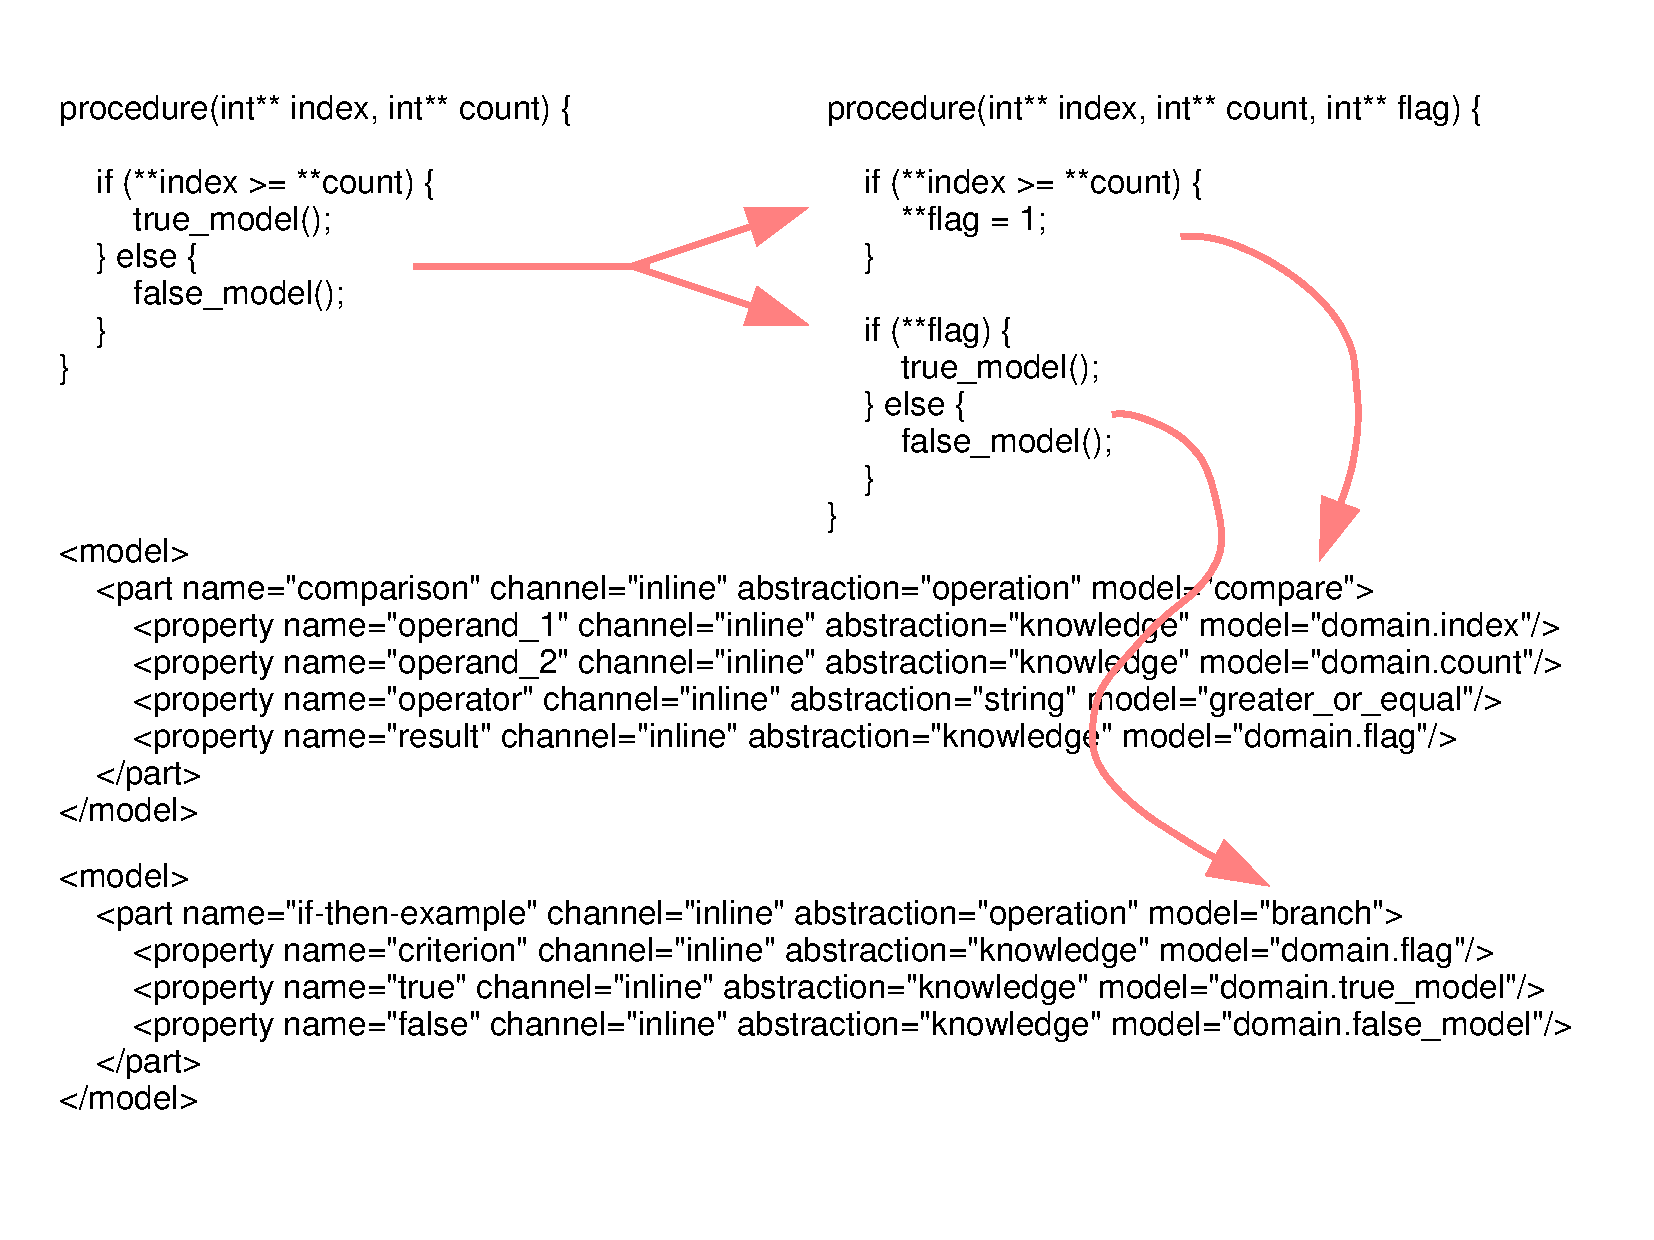
\includegraphics[scale=0.3,angle=-90]{graphics/cybolcondition.pdf}
        \caption{Condition Control Structure and Elements in C and CYBOL}
        \label{cybolcondition_figure}
    \end{center}
\end{figure}

Flags as one of the earliest techniques used in computing (in software as well
as in hardware) are the perfect means for controlling the execution of
primitive logic models, namely operations. They represent a condition set as
result of another logic model -- the latter often being some kind of comparison
operation. In order to execute code upon activation of a flag, a conventional
comparison control structure needs to be split up into two independent blocks
(figure \ref{cybolcondition_figure}), with the flag being the linking element.
The flag which was set by a comparison operation is used for branching the
control flow.

The second example shows how a classical \emph{if-then} statement would be
written in CYBOL. The corresponding operation is called \emph{branch} and it
expects three properties: a \emph{criterion} flag and two models, of which one
is executed in case the flag is \emph{true} and the other is executed otherwise.

\begin{scriptsize}
    \begin{verbatim}
<model>
    <part name="if-then-example" channel="inline" abstraction="operation" model="branch">
        <property name="criterion" channel="inline" abstraction="knowledge" model=".domain.flag"/>
        <property name="true" channel="inline" abstraction="knowledge" model=".domain.true_model"/>
        <property name="false" channel="inline" abstraction="knowledge" model=".domain.false_model"/>
    </part>
</model>
    \end{verbatim}
\end{scriptsize}

